\documentclass[12pt]{article}

\usepackage[ngerman]{babel}
\usepackage[utf8]{inputenc}
\usepackage[scale=0.80]{geometry}
\usepackage{amsmath}
\usepackage{amssymb}
\usepackage{graphicx}
\usepackage{fancyhdr}

\renewcommand{\familydefault}{\sfdefault}
\renewcommand{\arraystretch}{1.25}
\setlength{\headheight}{28pt}
\pagestyle{fancy}

\lhead{\textbf{Datenbanksysteme II}\\
\textbf{Lösung von Aufgabe 1}}
\rhead{\textbf{Felix Wolff, Markus Petrykowski}\\
\textbf{Übungsgruppe B}}
\renewcommand{\footrulewidth}{0pt}

\begin{document}
\textbf{1 a)}
\begin{center}
    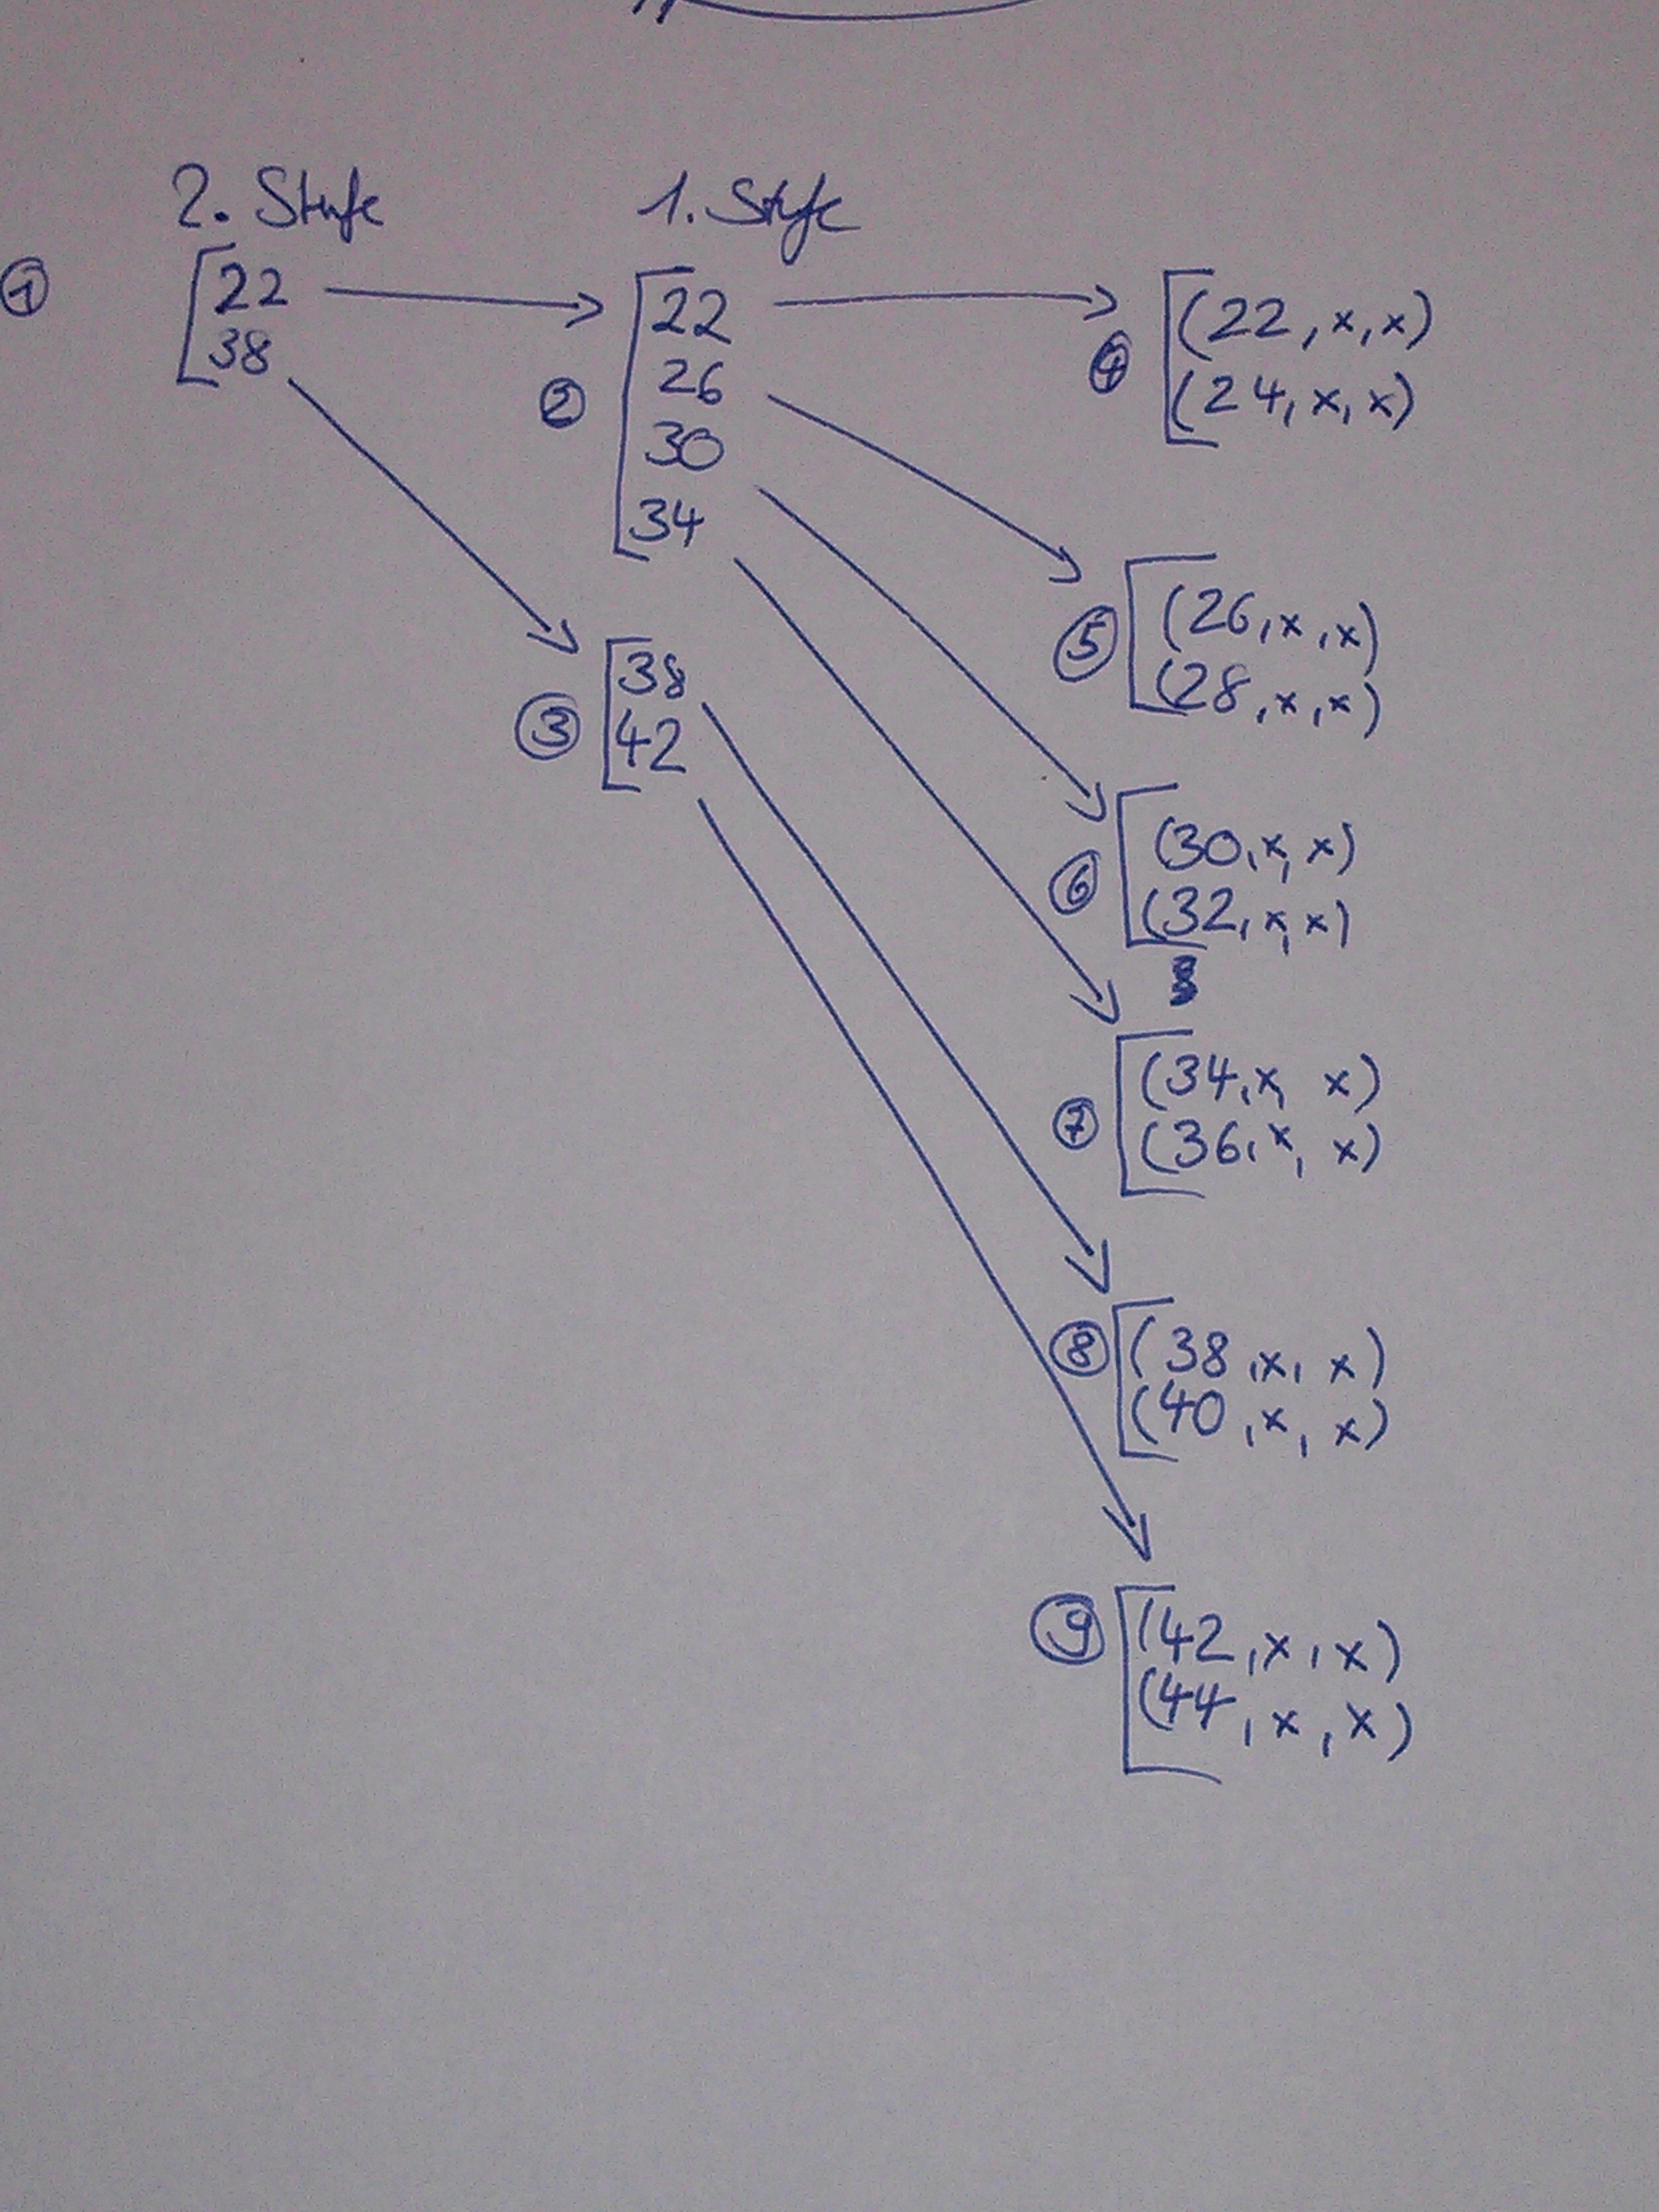
\includegraphics[scale=0.1]{index.jpg}
\end{center}

\textbf{1 b)}
\begin{enumerate}
    \item 1;2;7 - Über die zwei Indexstufen wird direkt zum Block mit $A=34$ gesprungen
    \item 1;2;7;8;9 - Ab diesem Block wird die Datei nach unten durchlaufen, da sie
        sequentiell ist.
    \item 1 - denn A ist Primärschlüssel
    \item 1 - denn A ist Primärschlüssel
    \item 1 - Der Index ist auf einer sequentiellen Datei angeordnet worden,
        insofern befindet sich das kleinste $A$ ganz oben im Index
    \item 9 - Gleiche Überlegung wie bei \verb=MIN=, nur dass das größte $A$
        im letzten Block der Relation liegt. Ansonsten, falls das DBMS nicht
        genau weiß, wo die Datei endet ist die Reihenfolge 1;3;9.
    \item 4;5;6;7;8;9 - Zur Bildung des Durchschnitts ist der dünnbesetzte Index
        nutzlos, weswegen er gar nicht verwendet werden muss, sofern der Beginn
        der Relation bekannt ist.
\end{enumerate}
\end{document}
% vim: tw=80
